\documentclass[12pt]{article}

%\documentclass[17pt]{extarticle}

%\usepackage{extsizes}
\usepackage{indentfirst}
\usepackage[utf8x]{inputenc}
\usepackage[T1]{fontenc}
\usepackage[english,lithuanian]{babel}
\usepackage{array}
\usepackage{caption}
\usepackage{makecell}
\usepackage[euler]{textgreek}
\usepackage{hyperref}
\usepackage{multirow}
\usepackage{boldline}
\usepackage{floatrow}
\floatsetup[table]{capposition=top}

\usepackage{amsmath, amsthm, amssymb}
\usepackage{graphicx}
\usepackage{setspace}
\usepackage{verbatim}
\usepackage[left=3cm,top=2cm,right=1.5cm,bottom=2cm]{geometry}
\usepackage{floatrow}
\newfloatcommand{capbtabbox}{table}[][\FBwidth]
\usepackage{blindtext}

\onehalfspacing

\newcommand{\EE}{\mathbb{E}\,} % Mean
\newcommand{\ee}{{\mathrm e}}  % nice exponent
\newcommand{\dd}{{\mathrm d}}
\newcommand{\RR}{\mathbb{R}}

\begin{document}
\selectlanguage{lithuanian}

\begin{titlepage}
\vskip 20pt
\begin{center}

\includegraphics[scale=0.5]{MIF}
\end{center}

%%%%%%%%%%%%%%%%%%%%%%%%%%%%%%%%%%%%%%%%
% TITULINIO PUSLAPIO TEKSTAS
%%%%%%%%%%%%%%%%%%%%%%%%%%%%%%%%%%%%%%%%

\vskip 20pt
\centerline{\bf \large \textbf{VILNIAUS UNIVERSITETAS}}
\bigskip
\centerline{\large \textbf{MATEMATIKOS IR INFORMATIKOS FAKULTETAS}}
\bigskip
\centerline{\large \textbf{BIOINFORMATIKOS BAKALAURO STUDIJŲ PROGRAMA}}

\vskip 90pt
\begin{center}
    {\bf \LARGE \emph{tbx5} ir \emph{tcf21} genų įtakos regeneracijai tyrimai}
\end{center}
\begin{center}
    {\bf \Large Research of the \emph{tbx5} and \emph{tcf21} genes' functions in regeneration}
\end{center}
\vskip 20pt
\centerline{\bf \large \textbf{Kursinis darbas}}
\bigskip
\vskip 50pt

\hskip 140pt {\large Autorius: Danielė Stasiūnaitė}

\hskip 140pt{\large VU el. p.: (daniele.stasiunaite@mif.stud.vu.lt)}
\bigskip
\vskip 20pt

\hskip 140pt {\large Darbo vadovas: J. m. d. Kotryna Kvederavičiūtė}
\vskip 60pt
\vskip 60pt
\centerline{\large \textbf{Vilnius}}
\centerline{\large \textbf{2022}}
\newpage
\end{titlepage}

\selectlanguage{lithuanian}

%%%%%%%%%%%%%%%%%%%%%%%%%%%%%%%%%%%%%%%%
% TURINIO PUSLAPIS
%%%%%%%%%%%%%%%%%%%%%%%%%%%%%%%%%%%%%%%%  
\tableofcontents
\newpage

%%%%%%%%%%%%%%%%%%%%%%%%%%%%%%%%%%%%%%%%
% LIETUVIŠKOS SANTRAUKOS PUSLAPIS
%%%%%%%%%%%%%%%%%%%%%%%%%%%%%%%%%%%%%%%%  
\section*{Santrauka}
Darbo santrauka.\\

\textbf{Raktiniai žodžiai: ChIP-seq, TF, Tbx5, regionas, motyvas, R}
\newpage

%%%%%%%%%%%%%%%%%%%%%%%%%%%%%%%%%%%%%%%%
% ANGLIŠKOS SANTRAUKOS PUSLAPIS
%%%%%%%%%%%%%%%%%%%%%%%%%%%%%%%%%%%%%%%%
\section*{Summary}
Short summary of results.\\

\textbf{Keywords: ChIP-seq, TF, Tbx5, peak, motif, R}
\newpage

%%%%%%%%%%%%%%%%%%%%%%%%%%%%%%%%%%%%%%%%
% ĮVADO PUSLAPIS
%%%%%%%%%%%%%%%%%%%%%%%%%%%%%%%%%%%%%%%%
\section{Įvadas}
\newpage

%%%%%%%%%%%%%%%%%%%%%%%%%%%%%%%%%%%%%%%%
% DUOMENŲ APŽVALGA
%%%%%%%%%%%%%%%%%%%%%%%%%%%%%%%%%%%%%%%%
\section{Duomenų bazės ir duomenys}
\subsection{GTRD duomenų bazė}
Tyrimui naudoti duomenys atsisiųsti iš GTRD
(Gene Transcription Regulation Database)\cite{GTRD}
duomenų bazės, saugančios informaciją apie transkripcijos
sekų ir atviro chromatino regionus. Taip pat duomenų bazėje saugomi
nekartografuojamų regionų duomenys bei potencialūs žmonių bei naminių
pelių regionai, prie kurių gali jungtis transkripcijos faktoriai.

Ši duomenų bazė pasirinkta dėl sistemiškai surinktų
ChIP-seq eksperimentų, kurių metu gauti rezultatai yra unifikuotai
apdoroti ir paruošti tyrėjų meta-analizėms.

GTRD duomenų bazėje duomenys saugomi binariniu anotacijų
formatu \emph{bigBed}, leidžiančiu atvaizduoti pasirinktą
chromosomos regioną interaktyviose genominės informacijos
vizualizavimo naršyklėse (pavyzdžiui, UCSC Genome Browser\cite{UCSCGB})
efektyviau nei tekstinis BED formatas.

\subsection{Pasirinktų mėginių charakteristika}
Analizė atlikta, naudojantis 4 nepriklausomais eksperimentais, kuriuos
iš viso sudarė 7 biologinės replikos.
Pirmoje lentelėje pateikta informacija apie tyrimui atlikti
naudotus duomenis, surinktus iš naminės pelės (\emph{lot. Mus musculus})
ląstelių.

\begin{table}[htb]
    \newcolumntype{M}[1]{>{\centering\arraybackslash}m{#1}}
    \small
    \caption*{\textbf{1 lentelė.} \emph{Mėginių charakteristikos}}
    \begin{tabular}{|c|c|c|c|c|c|c|}
    \hline
    %\thead{Sample\\ window}
    \textbf{GTRD ID} & \textbf{Ląstelių tipas} &
        \textbf{\thead{Kamienas}} & \textbf{\thead{Poveikis}} &
        \textbf{Antikūnai} & \textbf{PubMed ID}\\
    \hline
    EXP030898 & \thead{HL - 1\\ (širdies raumens)} &
                C57BL/6J & \thead{TRE\\ promotorius (2 d.)} &
                - & 21415370\cite{ARTCL1}\\ 
    \hline
    EXP058852 & Širdies prieširdžių & C57BL/6 &
                - & \thead{Tbx5\\ (sc-17866)} & 31080136\cite{ARTCL2}\\
    \hline
    EXP062056 & \thead{Pelių naujagimių širdies\\ fibroblastų, 
                ekspresuojančių\\ didelį kiekį T antigeno, linija} &
                CD1 & \thead{sb431542,\\ xav939} &
                \thead{anti-TBX5\\ (sc-17866x)} & 31271750\cite{ARTCL3}\\
    \hline
    EXP058843 & \thead{MEF\\ (embrionų fibroblastai)} &
                C57BL/6 & AGHMT (2 d.) &
                \thead{anti-Tbx5\\ (sc-17866)} & 31080136\cite{ARTCL2}\\
    \hline
    EXP058847 & \thead{MEF\\ (embrionų fibroblastai)} &
                C57BL/6 & GHMT (2 d.) &
                \thead{Tbx5\\ (sc-17866)} & 31080136\cite{ARTCL2}\\
    \hline
    EXP058850 & \thead{MEF\\ (embrionų fibroblastai)} &
                C57BL/6 & GMT (2 d.) &
                \thead{Tbx5\\ (sc-17866)} & 31080136\cite{ARTCL2}\\
    \hline
    EXP058856 & \thead{MEF\\ (embrionų fibroblastai)} & 
                C57BL/6 & \thead{vienas\\ faktorius (2 d.)} &
                \thead{Tbx5\\ (sc-17866)} & 31080136\cite{ARTCL2}\\
    \hline
    \end{tabular}
\end{table}
\newpage

\subsection{Santrumpų bei pavadinimų paaiškinimai}
\begin{itemize}
    \item \textbf{HL - 1}: pelių širdies raumens ląstelės, išgautos
          iš navikinių prieširdžių kardiomiocitų linijos. Šios ląstelės
          gali betarpiškai dalintis ir spontaniškai keisti
          savo formą, vykstant širdies raumens susitraukimo/
          atsipalaidavimo procesams.
    \item \textbf{MEF}: pelių embrionų fibroblastai (\emph{angl.}
          Mouse Embryonic Fibroblast). Šiai ląstelių
          linijai būdingas ląstelių gyvybingumo apribojimas,
          reiškiantis, jog šios ląstelės greitai pasensta ir miršta.
    \item \textbf{C57BL/6}: inbrydingo (\emph{angl.} inbreeding) būdu
          išvestų naminių pelių veislė. Šios veislės pelėms
          būdingas itin tamsus kailis, padidėjęs jautrumas garsams,
          kvapams, skausmui ir žemai temperatūrai. Ši veislė
          dažnai naudojama nutukimą ir imuninę sistemą tiriančiuose
          tyrimuose.
    \item \textbf{C57BL/6J}: prie naminių pelių veislės pavadinimo
          pridėtos raidės patikslina, kurioje laboratorijoje veislės
          išvestos. 'J' raidė nurodo, kad pelių veislė išvesta Meino
          valstijoje (JAV) įsikūrusioje Džeksono laboratorijoje\cite{JCKSLAB}.
    \item \textbf{CD1}: autbrydingo (\emph{angl.} outbreeding) būdu
          išvestų naminių pelių veislė. Šios veislės pelėms
          būdingas baltas kailis. Taip pat CD1 pelės dažnai naudojamos
          genetiniuose, toksikologiniuose, farmakologiniuose ir
          senėjimo tyrimuose.
    \item \textbf{TRE}: tetraciklino atsako elementas (\emph{angl.} 
          Tetracycline Response Element). Tai yra 7 DNR sekos fragmentai,
          sudaryti iš 19 nukleotidų ir atskirti trumpesniais sekų
          fragmentais.
    \item \textbf{sb431542}: stipriai veikianti, selektyvi cheminė
          medžiaga; transformuojančio augimo faktoriaus {\textbeta}
          (TGF-{\textbeta}) inhibitorius.
    \item \textbf{xav939}: stipriai veikianti cheminė medžiaga;
          tankirazės inhibitorius. Tankirazė slopina TERF1 baltymo,
          stabdančio telomerazės veiklą, jungimąsi prie telomerinių
          DNR sekų.
    \item \textbf{AGHMT}: AKT1 - serino/treonino kinazė 1; GATA4,
          HAND2, MEF2C, \emph{Tbx5} - kardiogeniniai transkripcijos faktoriai.
    \item \textbf{GHMT}: GATA4, HAND2, MEF2C, TBX5 transkripcijos
          faktorių komplektas.
    \item \textbf{GMT}: GATA4, MEF2C, \emph{Tbx5}  transkripcijos
          faktorių komplektas.
    \item \textbf{sc-17866x/ sc-17866}: iš ožkų išskirti antikūnai,
    \     atpažįstantys žmonių, pelių ir žiurkių \emph{Tbx5} antigeną.
\end{itemize}


\subsection{Pasirinktų eksperimentų apžvalga}
\begin{itemize}
    \item \textbf{EXP030898}: vienas mėginys iš septyniolikos eksperimento
        metu tirtų mėginių. Eksperimente buvo siekiama patvirtinti arba
        atmesti hipotezę apie širdies stipriklių (\emph{angl.} enhancer)
        identifikiavimą prie chromatino jungiantis keliems transkripcijos
        faktoriams.

        HL - 1 širdies raumens ląstelės buvo infekuotos
        su adenovirusu, ekspresuojančiu troponiną T, kuris skatina
        \emph{rtTA} ir \emph{BirA} genų ekspresiją, bei TRE promotoriumi,
        skatinančiu \emph{Tbx5} transkripcijos faktoriaus geno raišką.
        Sąlygos taikytos 48 valandas.
    \item \textbf{EXP058852}: prieširdžių ląstelės buvo du kartus po 24
        valandas laikytos mišinyje su retrovirusais. Papildomi poveikiai
        nebuvo taikyti.
    \item \textbf{EXP062056}: eksperimente ląstelės buvo infekuotos su
        GATA4, Mef2c, ir \emph{Tbx5} transkripcijos faktorius sintetinančiais
        retrovirusais. Ląstelės augintos terpėje, kurioje buvo {Tgf\textbeta}
        inhibitoriaus sb431542, skatinančio kardiomiocitų diferenciaciją
        iš pliuripotentinių kamieninių ląstelių, ir Wnt inhibitoriaus
        xav939, stabdančio nediferencijuotų ląstelių sintezę ir
        skatinančio progenitorinių ląstelių kardiomiogenezę.
\end{itemize}

Pasirinktų duomenų rinkinyje naudoti vieno eksperimento, kuriame buvo
tirti širdies ląstelių atsinaujinimo ir diferenciacijos mechanizmai,
keturiais skirtingais poveikiais tirti mėginiai:

\begin{itemize}
    \item \textbf{EXP058843}: embrionų fibroblastai veikti AGHMT. Esant
        kardiogeniniams transkripcijos faktoriams, AKT1 skatina fibroblastų
        diferenciaciją į širdies ląsteles - kardiomiocitus.
    \item \textbf{EXP058847}: neįtraukta AKT1 serino/treonino kinazė 1.
    \item \textbf{EXP058850}: į kardiogeninių transkripcijos faktorių mišinį
        neįtrauktas HAND2 transkripcijos faktorius.
    \item \textbf{EXP058856}: ląstelės veiktos tik vienu faktoriumi, kuris
        straipsnyje nebuvo specifikuotas.
  \end{itemize}
\newpage

%%%%%%%%%%%%%%%%%%%%%%%%%%%%%%%%%%%%%%%%
% METODAI
%%%%%%%%%%%%%%%%%%%%%%%%%%%%%%%%%%%%%%%%

\section{Tyrimo metodai}
\emph{Tbx5} transkripcijos faktoriaus regionų tyrimo analizė atlikta
su R programavimo kalba\cite{R} (4.2.0 versija).

Tarpiniams analizės rezultatams pateikti naudotas komandinės eilutės
įrankis Scikick\cite{SCIK} (0.2.0 versija), leidžiantis generuoti
R Markdown (Rmd) ataskaitas \emph{html} formatu bei kurti
struktūrizuotus puslapius, apjungiant iš daugelio Rmd failų
gautus HTML ataskaitų failus.

\subsection{Regionų skaičiaus nustatymas mėginiuose}
\emph{Tbx5} regionų skaičius skirtinguose mėginiuose apskaičiuotas
su standartine R ilgio funkcija \emph{length()}, kuri pritaikyta
\emph{GRanges} objektui, aprašančiam genomines pozicijas bei su jomis
susijusias anotacijas. Objektas sukurtas su \emph{rtracklayer}\cite{R_TRACK}
bibliotekos funkcija \emph{import()}.
Regionų skaičių mėginiuose atvaizduojanti stulpelinė diagrama
sukurta su \emph{ggplot2}\cite{R_GGPLOT} bibliotekos
\emph{geom\_bar()} funkcija.

\subsection{Regionų skaičiaus nustatymas chromosomose}
Transkripcijos faktoriaus regionų skaičius skirtingose chromosomose
kiekvienam mėginiui apskaičiuotas, naudojantis standartine R
funkcija \emph{length()}, pritaikyta atskiroms chromosomoms,
kurių pozicijos aprašytos \emph{GRanges} objekte.
Kiekvieno mėginio \emph{Tbx5} transkripcijos faktoriaus pasiskirstymas
chromosomose atvaizduotas su \emph{ggplot()} ir papildoma funkcija
\emph{facet\_wrap()}, sukuriančia atskirus grafikus pagal pasirinktą
elementą - chromosomas.

\subsection{Persidengiančių regionų procentinė dalis}
Persidengiančių regionų tarp mėginių procentinė dalis nustatyta
su modifikuota \emph{Jaccard()} funkcija, apskaičiuojančia,
kiek yra sutampančių regionų tarp dviejų mėginių poros.
Naudojantis nemodifikuota funkcija, Jaccard koeficientas
apskaičiuojamas pagal išraišką:
\[ J(A, B) =  \frac{|A \cap B|}{|A \cup B|} \]

\emph{Jaccard} koeficientas gaunamas iš rinkiniams A ir B bendrų duomenų ilgio
padalinus dviejų duomenų rinkinių bendrą duomenų ilgį.

Modifikavus \emph{Jaccard} koeficiento gavimo funkciją, koeficientas
apskaičiuojamas pagal išraišką, kur sutampančių A ir B rinkinių
duomenų ilgis padalinamas iš A rinkinio ilgio:

\[ J(A, B) = \frac{|A \cap B|}{|A|} \]

\emph{Jaccard} koeficiento skaičiavimo funkcija modifikuota, nes
skaičiuojant koeficientą su standartine \emph{Jaccard} funkcija,
gaunamas itin didelis regionų sąjungos skaičius, o
persidengiančių regionų skaičius gaunamas mažas, todėl
persidengiančių regionų skaičių padalinus iš regionų sąjungos
gaunamas itin mažas koeficientas, kurio apskaičiuota procentinė
dalis neretai neviršijo 1\%.

Tam, jog būtų galima patikimiau įvertinti, kokia pirmojo mėginio
procentinė regionų dalis persidengia su antruoju mėginiu,
persidengiančių regionų skaičius padalintas iš pirmojo mėginio
regionų skaičiaus.

Gauti rezultatai atvaizduoti spalvų intensyvumo grafike (\emph{angl.}
heatmap), sukurtame su \emph{ggplot()} ir papildoma funkcija
\emph{geom\_tile()}.

\subsection{\emph{Tbx5} motyvo nustatymas}
Šiame etape genomines pozicijas aprašantys \emph{bigBed} formato
failai konvertuoti į BED formato failus, pasinaudojus
UCSC komandinės eilutės programa \emph{bigBedToBed}\cite
{BBTOBED}.

Sugeneruoti BED formato failai panaudoti pikus atitinkančių
sekų iš naminės pelės genomo gavimui FASTA formatu.
Sekos iš genomo išgautos, pasinaudojus komandinės eilutės įrankio
BEDTools\cite{BEDTOOLS}.
(2.30.0 versija) programa \emph{getfasta}\cite{GET_FASTA}.

Kiekviename mėginyje esančio \emph{Tbx5} transkripcijos faktoriaus
motyvo procentinė dalis apskaičiuota susumavus \emph{Biostrings}\cite{BIOSTR}
bibliotekos funkcijos \emph{countPWM()} rezultatus bei gautą
vertę padalinus iš bendro regionų skaičiaus.

Gauta \emph{Tbx5} transkripcijos faktoriaus procentinė dalis
vizualizuota su pagrindinėmis \emph{ggplot()} ir \emph{geom\_bar()}
funkcijomis.

\subsection{Motyvų paieška \emph{de novo}}
Praturtintų sekų radimui panaudota komandinės eilutės įrankio
HOMER\cite{HOMER} (v4.11 versija) programa
\emph{findMotifsGenome.pl},
analizuojanti BED formato failus (faile specifikuotas
pozicijas), ir ieškanti praturtintų sekų atitikimo anotuotame
naminės pelės \emph{mm10} referentiniame genome.
Tarp mėginių persidengiantys motyvai nustatyti, naudojantis
R biblioteka \emph{UpSetR}\cite{UPSETR}.

\subsection{Praturtintų sekų biologinių funkcijų nustatymas}
Identifikuotų motyvų biologinės funkcijos nustatytos, pasinaudojus
UniProt\cite{UNIPROT} duomenų bazės genų ontologijos
(\emph{angl.} Gene Ontology (GO))
biologinių procesų, ląstelinių komponentų ir molekulinių funkcijų
klasifikacija.

\newpage

%%%%%%%%%%%%%%%%%%%%%%%%%%%%%%%%%%%%%%%%
% GAUTŲ REZULTATŲ APŽVALGA
%%%%%%%%%%%%%%%%%%%%%%%%%%%%%%%%%%%%%%%%

%%%%%%%%%%%%%%%%%%%%%%%%%%%%%%%%%%%%%%%%
% REGIONŲ SKAIČIUS MĖGINIUOSE
%%%%%%%%%%%%%%%%%%%%%%%%%%%%%%%%%%%%%%%%
\section{Rezultatai ir jų aptarimas}
\subsection{Regionų skaičiaus skirtumai tarp mėginių}
Pirmajame analizės etape kiekviename mėginyje nustatytas bendras
regionų skaičius pavaizduotas pirmoje stulpelinėje diagramoje
(1 pav.).

\begin{figure}[htb]
    \begin{center}
        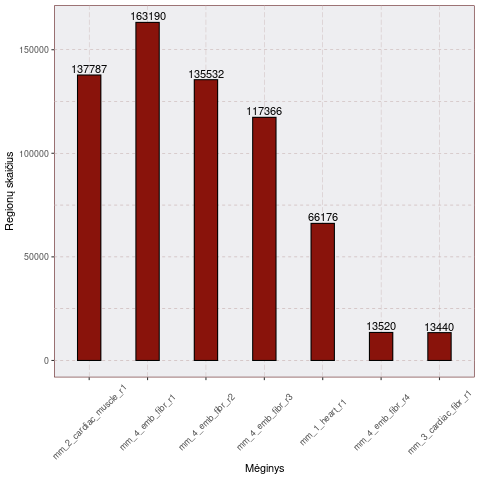
\includegraphics[width=0.7\linewidth]{Figures/total_peak_counts.png}
        \caption*{\textbf{1 pav.} \emph{Regionų skaičių kiekviename mėginyje
        vaizduojanti stulpelinė diagrama}}
    \end{center}
\end{figure}

Remiantis diagrama didžiausias \emph{Tbx5} transkripcijos faktoriaus
regionų skaičius nustatytas eksperimento \textbf{mm\_4\_emb\_fibr\_r1}
biologinėje replikoje, kurioje pelių embrionų fibroblastų ląstelės
dvi dienas veiktos AGHMT faktoriais.
Šį rezultatą palyginus su kitomis biologinėmis replikomis, kuriose
tirtas tas pats pelių embrionų fibroblastų ląstelių kamienas, tačiau
ląstelės veiktos tik kai kuriais faktoriais, pastebimas gradualus
\emph{Tbx5} transkripcijos faktoriaus regionų skaičiaus mažėjimas
diagramoje \textbf{mm\_4\_emb\_fibr\_r2}, \textbf{mm\_4\_emb\_fibr\_r3} ir
\textbf{mm\_4\_emb\_fibr\_r4} pavaizduotuose stulpeliuose.

Mėginyje, kuriame embrionų fibroblastai veikti tik vienu faktoriumi,
\emph{Tbx5} transkripcijos faktoriaus regionų nustatyta nedaug -
13520.

Mažiausiai regionų nustatyta mėginyje, kuriame tirta pelių
naujagimių širdies fibroblastų, ekspresuojančių T antigeną
ir paveiktų inhibitoriais: sb431542 ir xav939.
Nepaisant to, kad abu inhibitoriai skatina širdies ląstelių
diferenciaciją\cite{HEART_CELL_DIFF_ARTCL}, itin mažas transkripcijos
faktoriaus regionų skaičius rodo, kad papildomas veikimas
inhibitoriais daro mažą įtaką transkripcijos faktoriaus
jungimuisi prie DNR sekų.

\newpage

%%%%%%%%%%%%%%%%%%%%%%%%%%%%%%%%%%%%%%%%%%%%%
% REGIONŲ SKAIČIUS ATSKIROSE CHROMOSOMOSE
%%%%%%%%%%%%%%%%%%%%%%%%%%%%%%%%%%%%%%%%%%%%%
\subsection{Regionų pasiskirstymas chromosomose}
Nustačius \emph{Tbx5} transkripcijos faktoriaus regionų
pasiskirstymą eksperimentų mėginiuose, kitame analizės etape
patikrinta, kaip faktoriaus regionai pasiskirstę atskirose
chromosomose.

Vaizduojamuose grafikuose (2 pav.) didžiausias regionų skaičius nustatomas
pirmoje, antroje ir penktoje chromosomose. Naminės pelės pirmoji
chromosoma yra pati didžiausia, turinti 195 milijonų bazių porų,
antroji chromosoma sudaryta iš 182 megabazių, penktoji chromosoma -
152 milijonų bazių porų, todėl didesnis regionų skaičius šiose
chromosomose nėra neįprastas reiškinys. Kitose chromosomose regionų
skaičius yra mažesnis. Ypač mažas regionų skaičius nustatytas
devynioliktoje (61 Mbp), X (169 Mbp) ir Y (91 Mbp) chromosomose.

\begin{figure}[htb]
    \begin{center}
        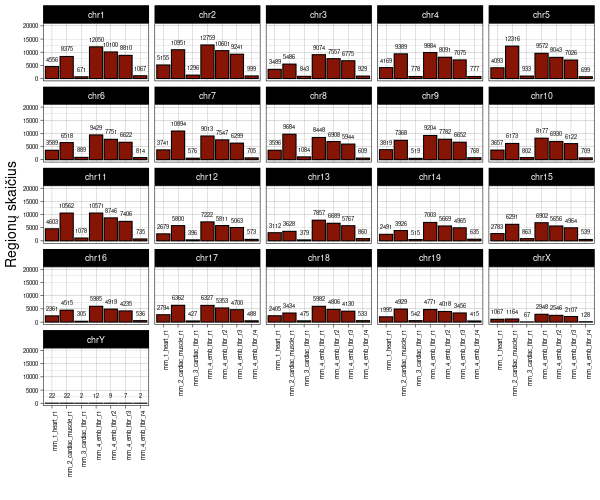
\includegraphics[width=0.8\linewidth]{Figures/peak_counts_by_chromosome.png}
        \caption*{\textbf{2 pav.} \emph{Regionų pasiskirstymas chromosomose}}
    \end{center}
\end{figure}

Biologinių replikų mėginiuose didžiausias regionų skaičius
nustatytas antroje chromosomoje. Taip pat grafikuose išsiskiria
kontrolinis HL - 1 širdies ląstelių mėginys, kuriame didžiausias
regionų skaičius nustatytas penktojoje chromosomoje.

Remiantis pavaizduotomis regionų skaičiaus pasiskirstymo
chromosomose stulpelinėmis diagramomis, itin išsiskiriantis
atrankumas chromosomų atžvilgiu nenustatytas, todėl galima
teigti, jog šiame analizės etape duomenų problematiškumas
nepastebimas arba jo nėra.

\newpage

%%%%%%%%%%%%%%%%%%%%%%%%%%%%%%%%%%%%%%%%%%%%
% TARP MĖGINIŲ PERSIDENGIANTYS REGIONAI
%%%%%%%%%%%%%%%%%%%%%%%%%%%%%%%%%%%%%%%%%%%%
\subsection{Tarp mėginių persidengiantys regionai}
Dažnai siekiant nustatyti mėginių panašumą, yra tiriama, kokia
mėginių duomenų dalis persidengia.

\begin{figure}[htb]
    \begin{center}
        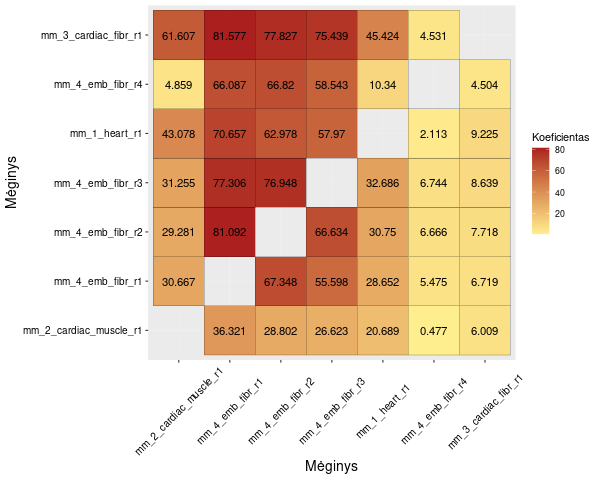
\includegraphics[width=0.8\linewidth]{Figures/peak_overlaps_between_samples.png}
        \caption*{\textbf{3 pav.} \emph{Persidengiančių regionų procentinės
                  dalies vaizdavimas}}
    \end{center}
\end{figure}

Remiantis pavaizduoto spalvų intensyvumo grafiko (3 pav.)
duomenimis, didžiausi persidengiančių regionų procentai
nustatyti tarp šių mėginių:
\begin{itemize}
    \item \textbf{81.577 \%} - tarp mėginio, kuriame buvo tiriamos širdies
            fibroblastų ląstelės, ekspresuojančios T antigeną, ir mėginio,
            kuriame tirti embrionų fibroblastai, veikiant AGHMT.
    \item \textbf{81.092 \%} - tarp mėginio, kuriame tirti embrionų
            fibroblastai ir mėginio, kuriame nebuvo AKT1.
    \item \textbf{77.827 \%} - tarp mėginio su T antigeną ekspresuojančiomis
            širdies fibroblastų ląstelėmis ir mėginio, kuriame nebuvo AKT1.
    \item \textbf{76.948 \%} - tarp mėginio, kuriame nebuvo HAND2
            faktoriaus, ir mėginio, kuriame nebuvo AKT1.
    \item \textbf{75.439 \%} - tarp mėginio su T antigeną ekspresuojančiomis
            širdies fibroblastų ląstelėmis ir tarp mėginio, kuriame nebuvo HAND2
            faktoriaus.
  \end{itemize}

%%%%%%%%%%%%%%%%%%%%%%%%%%%%%%%%%%%%
% TBX5 MOTYVO NUSTATYMAS
%%%%%%%%%%%%%%%%%%%%%%%%%%%%%%%%%%%%
\subsection{\emph{Tbx5} motyvo pasiskirstymas mėginiuose}
Ketvirtajame grafike (4 pav.) vaizduojama, kiek \emph{Tbx5}
motyvo atitikimų nustatyta skirtinguose mėginiuose.
<PAPILDYTI, NURODANT, KOKS TBX5 MOTYVAS BUVO NUSTATYTAS IR PAN.>

\begin{figure}[htb]
    \begin{center}
        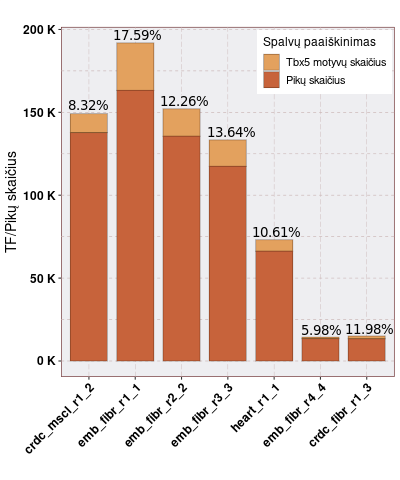
\includegraphics[width=0.7\linewidth]{Figures/tf_hit_percentage.png}
        \caption*{\textbf{4 pav.} \emph{Tbx5 motyvų atitikimų skaičiaus palyginimo
                  sudėtinė diagrama}}
    \end{center}
\end{figure}

Antroje lentelėje (2 lentelė) nurodoma, kokią procentinę dalį
tarp visų mėginių regionų sudaro \emph{Tbx5} motyvai.

\begin{table}[htb]
    \newcolumntype{M}[1]{>{\centering\arraybackslash}m{#1}}
    \small
    \caption*{\textbf{2 lentelė.} \emph{Mėginių charakteristikos}}
    \begin{tabular}{|c|c|}
    \hline
    \textbf{Mėginys} & \textbf{Procentinė dalis}\\
    \hline
        \textbf{mm\_2\_cardiac\_muscle\_r1} & 8.32\%\\ 
    \hline
        \textbf{mm\_4\_emb\_fibr\_r1} & 17.59\%\\
    \hline
        \textbf{mm\_4\_emb\_fibr\_r2} & 12.26\%\\
    \hline
        \textbf{mm\_4\_emb\_fibr\_r3} & 13.64\%\\
    \hline
        \textbf{mm\_1\_heart\_r1} & 10.61\%\\
    \hline
        \textbf{mm\_4\_emb\_fibr\_r4} & 5.98\%\\
    \hline
        \textbf{mm\_3\_cardiac\_fibr\_r1} & 11.98\%\\
    \hline
    \end{tabular}
\end{table}

\newpage

\subsection{\emph{De novo} identifikuoti motyvai}
\emph{De novo} motyvų paieškos programos įvykdymas buvo
ilgiausiai trukęs analizės etapas, lyginat su kitais 
tyrimo žingsniais. Šio etapo metu buvo sugeneruoti HTML
formato failai, kuriuose buvo pateiktas identifikuotų motyvų sąrašas,
išrikiuotas pagal p-vertę didėjančia tvarka, motyvų sekų logotipai,
nuorodos į puslapius su pozicinėmis motyvų svorių matricomis bei
identifikuotų motyvų procentinę dalį visame mėginio sekų rinkinyje,
pateiktame FASTA formatu.

Trečioje lentelėje (3 lentelė) kiekvienam mėginiui pavaizduoti trys
motyvai, turintys mažiausią p-vertę bei apimantys didžiausią mėginių
pilno sekų rinkinio dalį (procentiškai). Penktame trečios lentelės
stulpelyje nurodyta, kokią procentinę dalį mėginyje sudaro
identifikuotas \emph{Tbx5} motyvas.

\begin{table}[htb]
    \newcolumntype{M}[1]{>{\centering\arraybackslash}m{#1}}
    \small
    \caption*{\textbf{3 lentelė.} \emph{Identifikuotų motyvų pavyzdžiai}}
    \begin{tabular}{|c|c|c|c|c|}
    \hline
    \textbf{Mėginys} & \textbf{Pavadinimas} & \textbf{p vertė} &
                       \textbf{\thead{Procentinė\\ dalis}} &
                       \textbf{\emph{Tbx5} motyvas}\\
    \hlineB{2.5}
    \multirow{3}{*}{\textbf{mm\_2\_cardiac\_muscle\_r1}} &
                    Tbx6(T-box) & 1e-1881 & 20.28\% &
                    \multirow{3}{*}{\thead{1e-3266;\\ 54.87\%}} \\
    \cline{2-4}           & Tbet(T-box) & 1e-1472 & 16.48\% & \\
    \cline{2-4}           & Eomes(T-box) & 1e-1332 & 25.49\% & \\
    \hlineB{2.5}
    \multirow{3}{*}{\textbf{mm\_4\_emb\_fibr\_r1}} &
                    Mef2b(MADS) & 1e-3037 & 15.60\% &
                    \multirow{3}{*}{\thead{1e-2359;\\ 44.22\%}}\\
    \cline{2-4}           & TRPS1(Zf) & 1e-2983 & 31.99\% & \\
    \cline{2-4}           & GATA3(Zf) & 1e-2936 & 25.49\% & \\
    \hlineB{2.5}
    \multirow{3}{*}{\textbf{mm\_4\_emb\_fibr\_r2}} &
                    Fos(bZIP) & 1e-2912 & 13.22\% &
                    \multirow{3}{*}{\thead{1e-1873;\\ 42.97\%}}\\
    \cline{2-4}           & Fra1(bZIP) & 1e-2889 & 12.66\% & \\
    \cline{2-4}           & Fra2(bZIP) & 1e-2855 & 11.36\% & \\
    \hlineB{2.5}
    \multirow{3}{*}{\textbf{mm\_4\_emb\_fibr\_r3}} &
                    GATA3(Zf) & 1e-1895 & 25.06\% &
                    \multirow{3}{*}{\thead{1e-1391;\\ 41.04\%}}\\
    \cline{2-4}              & TRPS1(Zf) & 1e-1872 & 31.55\% & \\
    \cline{2-4}              & Fos(bZIP) & 1e-1857 & 11.66\% & \\
    \hlineB{2.5}
    \multirow{3}{*}{\textbf{mm\_1\_heart\_r1}} &
                    Mef2c(MADS) & 1e-1226 & 8.45\% &
                    \multirow{3}{*}{\thead{1e-438;\\ 39.08\%}}\\
    \cline{2-4}              & Mef2b(MADS) & 1e-1174 & 12.63\% & \\
    \cline{2-4}              & Mef2d(MADS) & 1e-1174 & 5.42\% & \\
    \hlineB{2.5}
    \multirow{3}{*}{\textbf{mm\_4\_emb\_fibr\_r4}} &
                    TRPS1(Zf) & 1e-1404 & 63.53\% &
                    \multirow{3}{*}{-}\\
    \cline{2-4}              & GATA3(Zf) & 1e-1271 & 52.43\% & \\
    \cline{2-4}              & GATA4(Zf) & 1e-1024 & 38.94\% & \\
    \hlineB{2.5}
    \multirow{3}{*}{\textbf{mm\_3\_cardiac\_fibr\_r1}} &
                    Tbx6(T-box) & 1e-1431 & 38.28\% &
                    \multirow{3}{*}{\thead{1e-1474;\\ 69.71\%}}\\
    \cline{2-4}              & Tbet(T-box) & 1e-1077 & 33.27\% & \\
    \cline{2-4}              & Tbx21(T-box) & 1e-1034 & 30.60\% & \\
    \hline
    \end{tabular}
\end{table}

Remiantis trečios lentelės duomenimis bei naudojantis statistinių
hipotezių testavimu itin mažos \emph{p} vertės rodo, jog tikimybė,
kad identifikuoti motyvai atsitiktiniai, yra labai maža, todėl
gauti duomenys yra statistiškai reišmingi - juos galima toliau
analizuoti.

Pirmajame ir paskutiniame mėginiuose, kurie lentelėje 
pažymėti \textbf{mm\_2\_cardiac\_muscle\_r1} ir
\textbf{mm\_3\_cardiac\_fibr\_r1}, \emph{Tbx5} motyvo \emph{p}
vertės buvo mažiausios, o procentinė dalis - didžiausia. Palyginus
šių mėginių rezultatus su 4.4 dalyje gautais tų pačių mėginių
rezultatais pastebimas didelis procentinės dalies neatitikimas,
tačiau šie procentai apskaičiuoti, naudojantis skirtingais
metodais. Taip pat 4.4 dalyje naudota pozicinė svorių
matrica neatitinka šioje dalyje identifikuoto \emph{Tbx5}
motyvo pozicinės svorių matricos.

Penktoje stulpelinėje diagramoje (5 pav.) vaizduojamas
bendras identifikuotų motyvų skaičius kiekvienam mėginiui.

\begin{figure}[htb]
    \begin{center}
        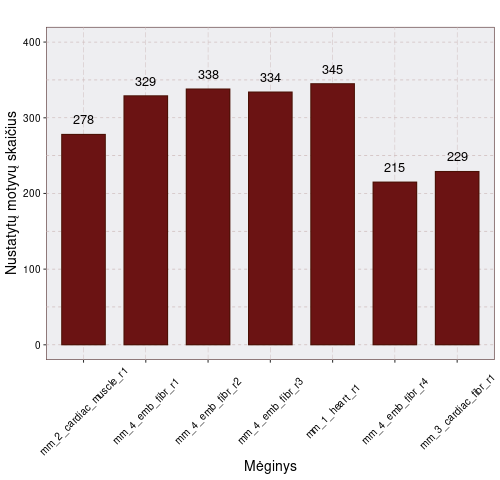
\includegraphics[width=0.7\linewidth]{Figures/motifs_in_samples.png}
        \caption*{\textbf{5 pav.} \emph{Identifikuotų motyvų skaičius mėginiuose}}
    \end{center}
\end{figure}

Nėra neįprasta, kad paskutinių mėginių (\textbf{mm\_4\_emb\_fibr\_r4} ir
\textbf{mm\_3\_cardiac\_fibr\_r1}) identifikuotų motyvų skaičius yra pats
mažiausias - šie mėginiai turi mažiausią regionų skaičių bei 
mažiausią juos atitinkančių sekų rinkinį.

Nepaisant šio atitikimo, mėginys \textbf{mm\_1\_heart\_r1}, turintis
mažiausią regionų skaičių po \textbf{mm\_4\_emb\_fibr\_r4} ir
\textbf{mm\_3\_cardiac\_fibr\_r1} mėginių, turi didžiausią identifikuotų
motyvų skaičių (345 motyvai). Nustatyti motyvai yra \( \sim \)12
nukleotidų ilgio.

Toliau pateikiamame grafike (6 pav.) vaizduojama, kiek vienodų
motyvų buvo nustatyta skirtinguose mėginiuose.

\newpage

\begin{figure}[htb]
    \begin{center}
        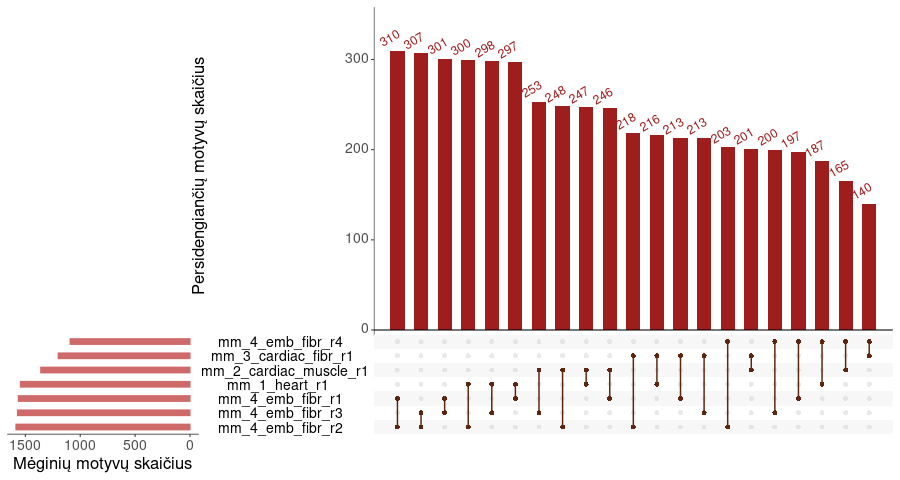
\includegraphics[width=1\linewidth]{Figures/motif_intersections.png}
        \caption*{\textbf{6 pav.} \emph{Tarp mėginių persidengiantys motyvai}}
    \end{center}
\end{figure}

Remiantis gautu grafiku, galima pastebėti, kad tarp mėginių porų
buvo nustatytas didelis visiems mėginiams būdingų motyvų skaičius.
Patikrinus, kiek motyvų aptinkami visuose mėginiuose, buvo nustatyta,
kad 131 motyvas yra būdingas visiems analizuojamiems mėginiams.

\subsection{\emph{De novo} nustatytų motyvų biologinės funkcijos}
Išsiaiškinus, kiek motyvų pateiktų mėginių regionų failuose buvo
identifikuota, buvo nustatytos su šiais motyvais susijusių genų
funkcijos.

Pateiktame funkcijų sąraše akronimas \textbf{MF} nurodo molekulinę
funkciją, \textbf{BP} - biologinį procesą, \textbf{CC} - ląstelės
komponentą. Naudojantis UniProtKB\cite{UNIPROTKB} duomenų bazės rezultatais,
visi trečioje lentelėje (3 lentelė) pateikti motyvai:

\begin{itemize}
    \item \textbf{MF:} atlieka jungimosi prie DNR funkciją bei
    dalyvauja transkripcijos procese.
    \item \textbf{BP:} dalyvauja ląstelių diferenciacijos
    procesuose.
    \item \textbf{CC:} yra aptinkami branduolyje.
\end{itemize}

\newpage

Unikalios motyvų funkcijos aprašytos sąraše:

\begin{enumerate}
    \item \textbf{Tbx6(T-box)\cite{TBX6} - T-box transkripcijos faktorius 6}
        \begin{itemize}
            \item \textbf{BP:} dalyvauja ląstelių proliferacijos
            ir organizacijos procesuose, signalinių kelių valdyme,
            kardioblastų diferenciacijoje.
            \item \textbf{CC:} nėra prisijungęs prie membranų,  
            aptinkamas branduolyje.
        \end{itemize}

    \item \textbf{Tbet(T-box)\cite{TBET} - T-box transkripcijos faktorius 21}
        \begin{itemize}
            \item \textbf{BP:} dalyvauja imuninės sistemos,
            baltymų metabolinių kelių procesuose. Taip pat
            pasireiškia organizmui reaguojant į dirgiklius.
            \item \textbf{CC:} aptinkamas branduolyje, neuroninių ląstelių kūne.
        \end{itemize}

    \item \textbf{Eomes(T-box)\cite{EOMES} - Eomesoderminas}
        \begin{itemize}
            \item \textbf{BP:} dalyvauja įvairių ląstelių (pavyzdžiui,
            kardiomiocitų) diferenciacijoje,
            neurogenezėje, kamieninių ląstelių populiacijos palaikyme
            \item \textbf{CC:} aptinkamas branduolyje, chromatine.
        \end{itemize}

    \item \textbf{Mef2b(MADS)\cite{MEF2B} - Miocitams specifiškas transkripcijos
                  aktyvatorius 2B}
        \begin{itemize}
            \item \textbf{BP:} dalyvauja įvairių ląstelių
            diferenciacijoje, transkripcijos proceso aktyvavime.
            \item \textbf{CC:} aptinkamas citozolyje, branduolyje,
            nukleoplazmoje, ląstelių jungtyse.
        \end{itemize}

    \item \textbf{Mef2c(MADS)\cite{MEF2C} - Miocitams specifiškas transkripcijos
                  aktyvatorius 2C}
        \begin{itemize}
            \item \textbf{BP:} dalyvauja ląstelių apoptozėje,
            kraujagyslių formavimęsi, pradinės embrionų
            širdies vystymęsi.
            \item \textbf{CC:} aptinkamas citozolyje, branduolyje,
            nukleoplazmoje, sarkomerose, sarkoplazmoje.
        \end{itemize}

    \item \textbf{Mef2d(MADS)\cite{MEF2D} - Miocitams specifiškas transkripcijos
                  aktyvatorius 2D}
        \begin{itemize}
            \item \textbf{BP:} dalyvauja suaugusių organizmų širdies
            vystymęsi, kremzlinių bei kaulinių ląstelių diferenciacijoje.
            \item \textbf{CC:} aptinkamas citoplazmoje, branduolyje,
            nukleoplazmoje.
        \end{itemize}

    \item \textbf{TRPS1(Zf)\cite{TRPS1} - Cinko „pirštelio” transkripcijos
                  faktorius}
        \begin{itemize}
            \item \textbf{BP:} dalyvauja kremzlinių ląstelių
            diferenciacijoje, skeleto vystymęsi, būdingas
            neigiamas transkripcijos reguliavimas.
            \item \textbf{CC:} aptinkamas branduolyje, nukleoplazmoje,
            chromatine, baltymų kompleksuose.
        \end{itemize}

    \item \textbf{GATA3(Zf)\cite{GATA3} - T ląstelėms specifiškas transkripcijos
                  faktorius GATA-3}
        \begin{itemize}
            \item \textbf{BP:} dalyvauja aortos vožtuvų formavimęsi,
            širdies prieširdžių morfogenezėje, embrionų organų
            vystymęsi, eritrocitų diferenciacijoje.
            \item \textbf{CC:} aptinkamas branduolyje, nukleoplazmoje,
            chromatine.
        \end{itemize}

    \item \textbf{GATA4(Zf)\cite{GATA4} - Transkripcijos faktorius GATA-4}
        \begin{itemize}
            \item \textbf{BP:} dalyvauja širdies ląstelių
            diferenciacijoje, širdies raumens regeneracijoje,
            embrionų širdies formavimęsi.
            \item \textbf{CC:} aptinkamas branduolyje, nukleoplazmoje,
            chromatine.
        \end{itemize}

    \item \textbf{Fos(bZIP)\cite{FOS} - AP-1 transkripcijos
                  faktoriaus subvienetas}
        \begin{itemize}
            \item \textbf{BP:} dalyvauja atsako į jonus (kadmio,
            kalcio), citokinus bei progesteroną procesuose. Taip
            pat aktyvus nervų sistemos vystymosi metu.
            \item \textbf{CC:} aptinkamas citozolyje, branduolyje,
            nukleoplazmoje, endoplazminiame tinkle, sinaptosomose.
        \end{itemize}

    \item \textbf{Fra1(bZIP)\cite{FRA1} - Onkogenas, AP-1 transkripcijos
                  faktoriaus subvienetas}
        \begin{itemize}
            \item \textbf{BP:} dalyvauja ląstelės ciklo valdyme,
            apoptoziniuose procesuose bei embrionų vystymosi
            gimdoje procesuose.
            \item \textbf{CC:} aptinkamas citozolyje, branduolyje,
            nukleoplazmoje, presinapsinėje membranoje.
        \end{itemize}

    \item \textbf{Fra2(bZIP)\cite{FRA2} - AP-1 transkripcijos
                  faktoriaus subvienetas}
        \begin{itemize}
            \item \textbf{BP:} dalyvauja teigiamoje fibroblastų
            proliferacijoje, atsako į estradiolio - moteriško
            lytinio hormono - procesuose. Taip pat būdinga
            teigiamas transkripcijos reguliavimas.
            \item \textbf{CC:} aptinkamas branduolyje ir
            nukleoplazmoje.
        \end{itemize}
\end{enumerate}

\newpage

%%%%%%%%%%%%%
% IŠVADOS
%%%%%%%%%%%%%

\section{Išvados}

\newpage

%%%%%%%%%%%%%%%%%%%%%%%%%%%%%%%%%%%%%%%%
% LITERATŪROS ŠALTINIAI
%%%%%%%%%%%%%%%%%%%%%%%%%%%%%%%%%%%%%%%%

\bibliographystyle{plain}
\begin{thebibliography}{99}

\bibitem{GTRD} GTRD: an integrated view of transcription regulation.
Kolmykov S, Yevshin I, Kulyashov M, Sharipov R, Kondrakhin Y, Makeev VJ,
Kulakovskiy IV, Kel A, Kolpakov F Nucleic Acids Res. 2021 Jan 8;49(D1):D104-D111.

\bibitem{UCSCGB} UCSC Genome Browser: Kent WJ, Sugnet CW, Furey TS, Roskin KM,
Pringle TH, Zahler AM, Haussler D. The human genome browser at UCSC. Genome Res.
2002 Jun;12(6):996-1006.

\bibitem{ARTCL1} He A, Kong SW, Ma Q, Pu WT. Co-occupancy by multiple cardiac
transcription factors identifies transcriptional enhancers active in heart.
Proc Natl Acad Sci U S A. 2011 Apr 5;108(14):5632-7. doi: 10.1073/pnas.1016959108.
Epub 2011 Mar 17. PMID: 21415370; PMCID: PMC3078411.

\bibitem{ARTCL2} Hashimoto H, Wang Z, Garry GA, Malladi VS, Botten GA, Ye W,
Zhou H, Osterwalder M, Dickel DE, Visel A, Liu N, Bassel-Duby R, Olson EN.
Cardiac Reprogramming Factors Synergistically Activate Genome-wide Cardiogenic
Stage-Specific Enhancers. Cell Stem Cell. 2019 Jul 3;25(1):69-86.e5.
doi: 10.1016/j.stem.2019.03.022. Epub 2019 May 9. PMID: 31080136;
PMCID: PMC6754266.

\bibitem{ARTCL3} Stone NR, Gifford CA, Thomas R, Pratt KJB, Samse-Knapp K,
Mohamed TMA, Radzinsky EM, Schricker A, Ye L, Yu P, van Bemmel JG, Ivey KN,
Pollard KS, Srivastava D. Context-Specific Transcription Factor Functions
Regulate Epigenomic and Transcriptional Dynamics during Cardiac Reprogramming.
Cell Stem Cell. 2019 Jul 3;25(1):87-102.e9. doi: 10.1016/j.stem.2019.06.012.
PMID: 31271750; PMCID: PMC6632093.

\bibitem{JCKSLAB} Jackson Laboratory (RRID:SCR\_004633).

\bibitem{R} R Core Team (2022).
R: A language and environment for statistical computing. R Foundation
for Statistical Computing, Vienna, Austria. URL https://www.R-project.org/.

\bibitem{SCIK}Scikick. Utility for executing collections
of computational notebooks.\\
URL https://petronislab.camh.ca/pub/scikick/stable/docs/report/out\_html/introduction.html

\bibitem{R_TRACK} M. Lawrence, R. Gentleman, V. Carey: "rtracklayer: an {R}
package for interfacing with genome browsers". Bioinformatics 25:1841-1842.

\bibitem{R_GGPLOT} H. Wickham. ggplot2: Elegant
Graphics for Data Analysis. Springer-Verlag New York, 2016.

\bibitem{BBTOBED} BigWig and BigBed tools: Kent WJ, Zweig AS, Barber G,
Hinrichs AS, Karolchik D. BigWig and BigBed: enabling browsing of large
distributed data sets. Bioinformatics. 2010 Sep 1;26(17):2204-7.

\bibitem{BEDTOOLS} Quinlan AR, Hall IM. BEDTools: a flexible suite of
utilities for comparing genomic features. Bioinformatics. 2010 Mar
15;26(6):841-2. doi: 10.1093/bioinformatics/btq033. Epub 2010 Jan 28.
PMID: 20110278; PMCID: PMC2832824.

\bibitem{GET_FASTA} BEDTools komandinės eilutės įrankis.
Programų rinkinio programa \emph{getfasta}.\\
Prieiga per https://bedtools.readthedocs.io/en/latest/content/tools/getfasta.html
[žiūrėta 2022-06-03].

\bibitem{BIOSTR} Pagès H, Aboyoun P, Gentleman R, DebRoy S (2022). \_Biostrings:
Efficient manipulation of biological strings\_. R package version
2.64.0, <https://bioconductor.org/packages/Biostrings>.

\bibitem{HOMER} Heinz S, Benner C, Spann N, Bertolino E et al.
Simple Combinations of Lineage-Determining Transcription Factors
Prime cis-Regulatory Elements Required for Macrophage and B Cell
Identities. Mol Cell 2010 May 28;38(4):576-589. PMID: 20513432.

\bibitem{UPSETR} Jake R. Conway, Alexander
Lex, Nils Gehlenborg. UpSetR: An R Package For The
Visualization Of Intersecting Sets And Their Properties
Bioinformatics, 33(18): 2938-2940,
doi:10.1093/bioinformatics/btx364, 2017.

\bibitem{UNIPROT} The UniProt Consortium
UniProt: the universal protein knowledgebase in 2021
Nucleic Acids Res. 49:D1 (2021).

\bibitem{UNIPROTKB} Boutet E, Lieberherr D, Tognolli M,
Schneider M, Bairoch A. UniProtKB/Swiss-Prot
Methods Mol. Biol. 406:89-112 (2007)

\bibitem{HEART_CELL_DIFF_ARTCL} Drowley L, Koonce C, Peel S, et al.
Human Induced Pluripotent Stem Cell-Derived Cardiac Progenitor
Cells in Phenotypic Screening: A Transforming Growth Factor-β
Type 1 Receptor Kinase Inhibitor Induces Efficient Cardiac
Differentiation. Stem Cells Transl Med. 2016;5(2):164-174.
doi:10.5966/sctm.2015-0114

\bibitem{TBX6} UniProtKB duomenų bazė. \emph{Tbx6 aprašymas} (2022).\\
Prieiga per https://www.uniprot.org/uniprot/P70327 [žiūrėta 2022-06-12].

\bibitem{TBET} UniProtKB duomenų bazė. \emph{Tbet aprašymas} (2022).\\
Prieiga per https://www.uniprot.org/uniprot/Q9JKD8 [žiūrėta 2022-06-12].

\bibitem{EOMES} UniProtKB duomenų bazė. \emph{Eomes aprašymas} (2022).\\
Prieiga per https://www.uniprot.org/uniprot/O54839 [žiūrėta 2022-06-12].

\bibitem{MEF2B} UniProtKB duomenų bazė. \emph{Mef2b aprašymas} (2022).\\
Prieiga per https://www.uniprot.org/uniprot/O55087 [žiūrėta 2022-06-12].

\bibitem{MEF2C} UniProtKB duomenų bazė. \emph{Mef2c aprašymas} (2022).\\
Prieiga per https://www.uniprot.org/uniprot/Q8CFN5 [žiūrėta 2022-06-12].

\bibitem{MEF2D} UniProtKB duomenų bazė. \emph{Mef2d aprašymas} (2022).\\
Prieiga per https://www.uniprot.org/uniprot/Q63943 [žiūrėta 2022-06-12].

\bibitem{TRPS1} UniProtKB duomenų bazė. \emph{TRPS1 aprašymas} (2022).\\
Prieiga per https://www.uniprot.org/uniprot/Q925H1 [žiūrėta 2022-06-12].

\bibitem{GATA3} UniProtKB duomenų bazė. \emph{GATA3 aprašymas} (2022).\\
Prieiga per https://www.uniprot.org/uniprot/P23772 [žiūrėta 2022-06-12].

\bibitem{GATA4} UniProtKB duomenų bazė. \emph{GATA4 aprašymas} (2022).\\
Prieiga per https://www.uniprot.org/uniprot/Q08369 [žiūrėta 2022-06-12].

\bibitem{FOS} UniProtKB duomenų bazė. \emph{Fos aprašymas} (2022).\\
Prieiga per https://www.uniprot.org/uniprot/P01101 [žiūrėta 2022-06-12].

\bibitem{FRA1} UniProtKB duomenų bazė. \emph{Fra1 aprašymas} (2022).\\
Prieiga per https://www.uniprot.org/uniprot/P48755 [žiūrėta 2022-06-12].

\bibitem{FRA2} UniProtKB duomenų bazė. \emph{Fra2 aprašymas} (2022).\\
Prieiga per https://www.uniprot.org/uniprot/P47930 [žiūrėta 2022-06-12].

\end{thebibliography}

\newpage

%%%%%%%%%%%%%%%%%%%%%%%%%%%%%%%%%%%%%%%%
% PRIEDAI
%%%%%%%%%%%%%%%%%%%%%%%%%%%%%%%%%%%%%%%%

\section{Priedas}

Priedų sąraše pateikiamos tarpinių rezultatų puslapio, sugeneruoto
su Scikick, bei Git repozitorijos, kurioje saugomi analizei naudoti
duomenų failai, parašyti skriptai bei pagrindinė R programa, nuorodos.

\begin{itemize}
    \item \textbf{Tarpinių rezultatų Scikick puslapis:}\\
        https://karklas.mif.vu.lt/\(\sim\)dast6577/KursinisDarbas/v1.1/peaks\_MM.html
    \item \textbf{Analizės Git repozitorija:}\\
        https://github.com/dansta0804/TF\_analysis.git
  \end{itemize}



\end{document}
